\section{Observation Notes}
\label{sec:appendix_observation_notes}

A number of relevant observations made by the authors as well as the seminar conductors and feedbacks from the participants during the three sessions are summarized in this listing – please note that in order to fully understand some of the following aspects, the reader should have seen the old version of the simulation:

\begin{itemize}
  \item \textbf{General:} Generally, the participants enjoyed playing the game and regard it as helpful to deepen their theoretical knowledge for example from the lecture ''Asset Management: Investments'' for Bachelor students. However, they regard the system as outdated and provided the authors with various ideas and critics. Decision data for a starting period 0 will be filled out by participants in Excel for a starting position before the seminar, afterward, they will be saved onto the USB drives for all teams by the seminar conductors. The seminar conductors will let the market model run and save its outcome back on the USB drive. This process is time-consuming and error-prone. In general, the participants think that it is difficult to make a decision in the first round, as too few information is available. More easily accessible comparative figures for the previous year would be helpful. Additionally, the stock selection is based on insufficient knowledge about the different titles.
  \item \textbf{Investment Process:} The given and to be kept bandwidths for the different asset class positions are not optimally placed and have to be looked up frequently. A temporary over-investment during the decision process is not possible and is always disturbed by pop-up windows.
  \item \textbf{Business Administration:} Various decisions regarding marketing, human resources as well as logistics are not very clear as especially in the beginning, the background and previous period information are not completely clear for the participants. The point here is, that a suitable level of abstraction has to be chosen as on the one hand, not every decision that has to be made in reality can be implemented in such a simplified simulation. On the one hand, a suitable number of decisions have to be enabled in order to support an appropriate learning effect.
  \item \textbf{Report:} The reports provided after each round of the game load very slowly and the comparison to other teams is cumbersome. It would be helpful if not only one group member can have the simulation and the reports on their screen. In general, more graphics are desired for better visualization of key aspects.
  \item \textbf{Teamwork:} The enabling of collaboration on several laptops within a team was mentioned many times. With today’s web-based technologies, much more implementation options are available.
\end{itemize}

The observation of the different players – students and practitioners, investment beginners and experts – allowed the project team to sense what the strengths and weaknesses of the old game are. Further, it helped to define an impact direction for the new game being developed, which resulted in another work model describing the process of the game based on its different phases.

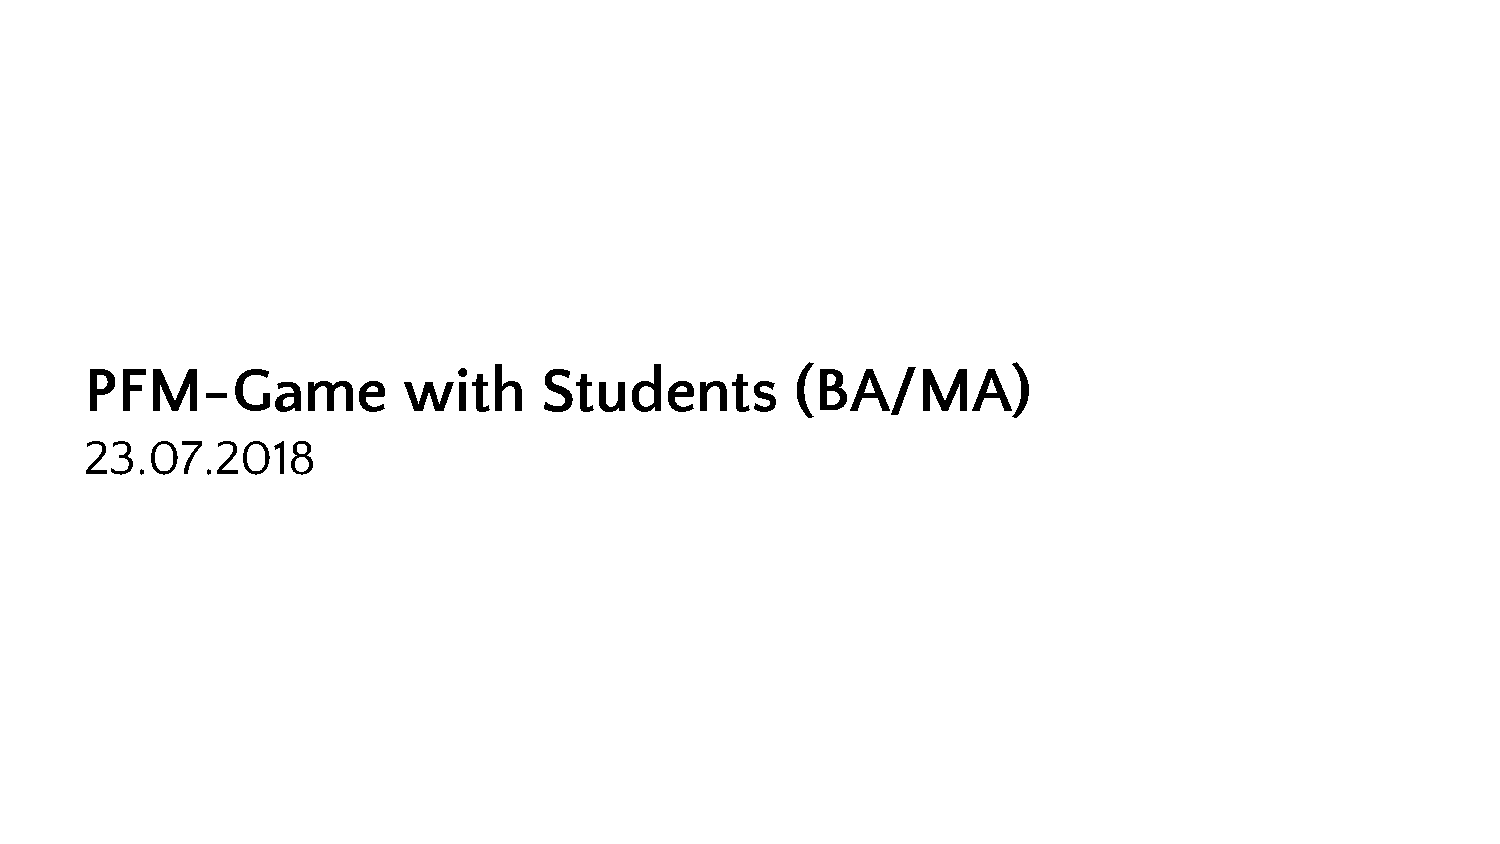
\includepdf[landscape=true, pages={-}, nup=1x2]{appendix/students_observation.pdf}

% TODO more about customer types etc.